\documentclass{beamer}
\usepackage[english]{babel}
\usepackage[utf8]{inputenc}
\usepackage[T1]{fontenc}
\usepackage{lmodern}
\usepackage{hus-beamer}
\usepackage{ifthen}
%\usetikzlibrary{intersections}
\usepackage[bibstyle=authoryear, citestyle=authoryear, maxcitenames=2, maxbibnames=2, backend=bibtex]{biblatex}
%\usepackage[maxbibnames=2]{biblatex}
%citestyle=authoryear or numeric or ...
\addbibresource{export.bib}

%------ tikZ ------%
\usepackage{tikz}
\usetikzlibrary{tikzmark,overlay-beamer-styles,babel} 
\usetikzlibrary{positioning, arrows}
\usetikzlibrary{backgrounds}
    
\mode<presentation>{
	\usefonttheme{professionalfonts} % normal font for math formulas
	% insert section page with title only
	% before each section
	\AtBeginSection[]{
	\begin{frame}%[noframenumbering] % remove this if you do not want to number section page
	\vfill
	\centering
	\begin{beamercolorbox}[sep=8pt,center,shadow=true,rounded=true]{title}
	\usebeamerfont{title}\insertsectionhead\par%
	\end{beamercolorbox}
	\vfill
	\end{frame}
}
}
%%%%%%%%
%\AtBeginBibliography{\footnotesize} % Footnotesize for Bibliography entries

% \setbeamertemplate{bibliography item}{%
%   \ifboolexpr{ test {\ifentrytype{book}} or test {\ifentrytype{mvbook}}
%     or test {\ifentrytype{collection}} or test {\ifentrytype{mvcollection}}
%     or test {\ifentrytype{reference}} or test {\ifentrytype{mvreference}} }
%     {\setbeamertemplate{bibliography item}[book]}
%     {\ifentrytype{online}
%        {\setbeamertemplate{bibliography item}[online]}
%        {\setbeamertemplate{bibliography item}[article]}}%
%   \usebeamertemplate{bibliography item}}

% \defbibenvironment{bibliography}
%   {\list{}
%      {\settowidth{\labelwidth}{\usebeamertemplate{bibli<title>ography item}}%
%       \setlength{\leftmargin}{\labelwidth}%
%       \setlength{\labelsep}{\biblabelsep}%
%       \addtolength{\leftmargin}{\labelsep}%
%       \setlength{\itemsep}{\bibitemsep}%
%       \setlength{\parsep}{\bibparsep}}}
%   {\endlist}
%   {\item}


%\defbibheading{bibliography}[\refname]{}

%------------------%

\begin{document}
\title{Common network architectures}
%\subtitle{Week 4}
\author{COMP6252 (Deep Learning Technologies)}
\institute[ECS, University of Southampton]{ECS, University of Southampton} 
\date{}
 \date{}
\begin{frame}[plain,noframenumbering]
    \placelogofalse % No logo at the title page
    \titlepage
\end{frame}
    
\placelogotrue
\begin{frame}
	\frametitle{Transfer learning}
\begin{itemize}
	
\item  Basically transfer learning is using pre-trained models
\item The model was already trained on a \textbf{different} datasets
\item The idea is the pre-trained network has learned "high level" features common to all images
\item  What is needed is some fine tuning
\item This is typically done by replacing the last layer of the pre-trained model
\item We will use the AlexNet model for illustration because it is not too big.
\item The idea is the same for all pre-trained networks
\end{itemize}
\end{frame}

\begin{frame}
    \frametitle{Replacing the last layer}
\begin{itemize}
    \item Almost all available (vision) models were trained on ImageNet competition
    \item The last layer outputs 1000 values
    \item We will use a model pre-trained on ImageNet to classify flowers (5 types)
\end{itemize}
\end{frame}


\begin{frame}
    \frametitle{Transfer learning}
\begin{center}
    \includegraphics[width=0.7\textwidth]{pdf/transfer-fig1.pdf}
\end{center}
\end{frame}


\begin{frame}
    \frametitle{Transfer learning}
\begin{center}
    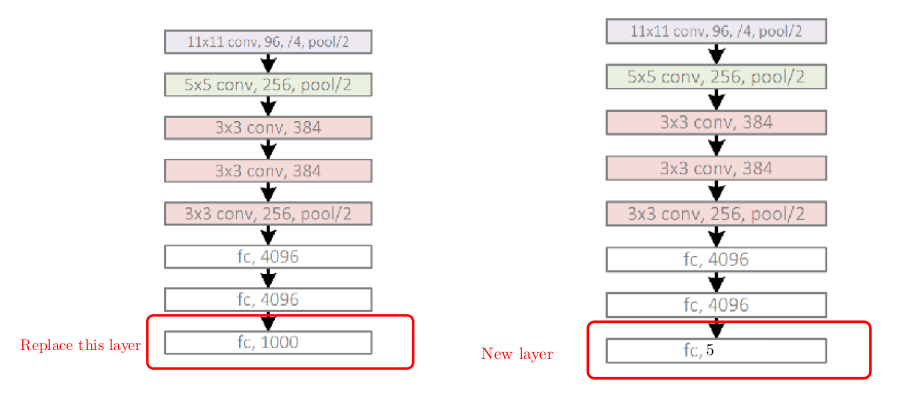
\includegraphics[width=\textwidth]{figs/transfer-fig4.png}
\end{center}
\end{frame}

\begin{frame}
    \frametitle{Why not start from scratch?}
    \begin{itemize}
        \item Validation accuracy vs epoch
        \item ResNet18 pre-trained (all layers): green
        \item ResNet18 trained with random initial weights: orange
    \end{itemize}
\begin{center}
    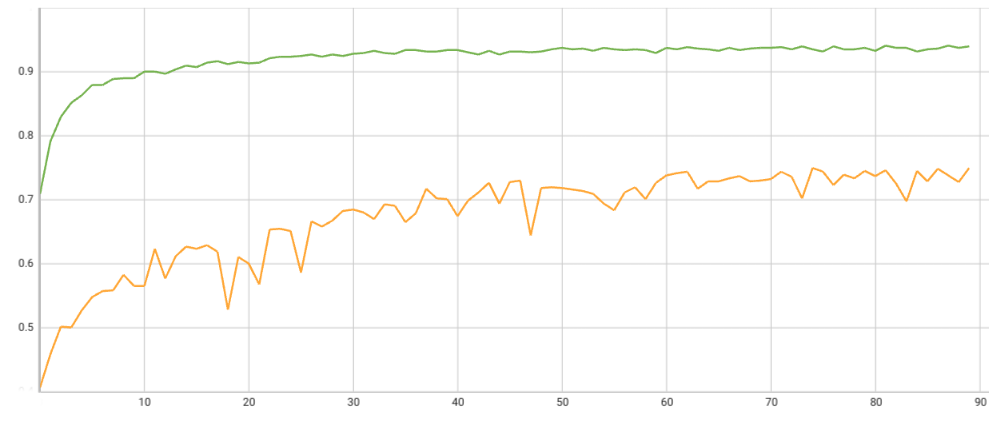
\includegraphics[width=\textwidth]{figs/pre-vs-scratch.png}
\end{center}
\end{frame}

\begin{frame}
    \frametitle{How to train a pre-trained model}
\begin{itemize}
    \item There are three approaches for training pre-trained models on a different dataset
    \begin{enumerate}
        \item "freeze" the weights of all intermediate layers and train the last layer
        \item train all the layers
        \item A hybrid approach where only the last layer is trained first followed by "unfreezing" the intermediate  layers
    \end{enumerate}
    \item The accuracy of different approaches is dataset dependent
\end{itemize}
    

\end{frame}



\begin{frame}
    \frametitle{Last vs all}
\begin{itemize}
    \item Validation accuracy vs epoch
    \begin{enumerate}
        \item All layers are trained: orange
        \item Only the last layer is trained (intermediate one are frozen): green
    \end{enumerate}
\end{itemize}
    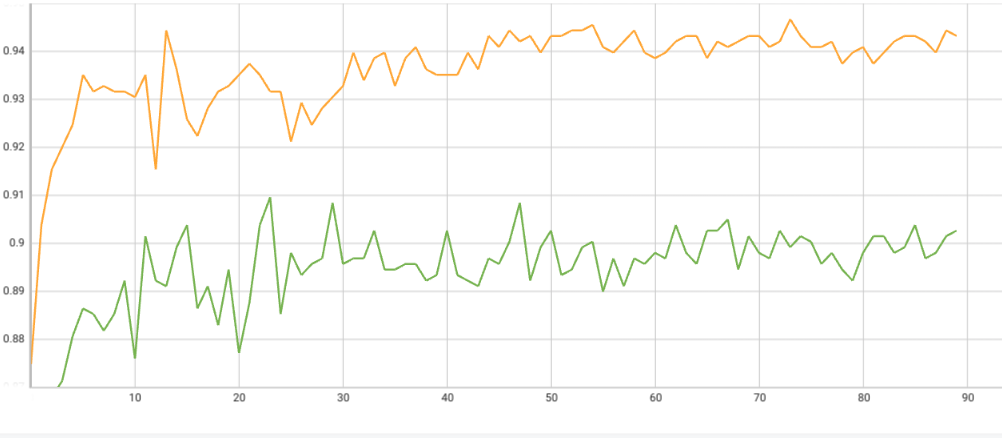
\includegraphics[width=\textwidth]{figs/last-vs-all.png}

\end{frame}

\begin{frame}
    \frametitle{SGD with momentum}

    \begin{itemize}
        \item A simple variant of SGD to reduce fast changing gradient
        \item It usually leads to better training convergence
        \item Let $w$ the learnable  be the weights and $\alpha$ the learning rate
        \item Instead of 
        \begin{align*}
            w=w-\alpha \nabla_w\mathcal{L}
        \end{align*}
\item use         
\begin{align*}
    dw&=\beta dw+(1-\beta)\nabla_w\mathcal{L}\\
    w&=w-\alpha dw
\end{align*}
\item where $\beta$ is a parameter, usually 0.9
    \end{itemize}
\end{frame}

\begin{frame}
    \frametitle{Why is it called moving average?}
    \begin{center}
        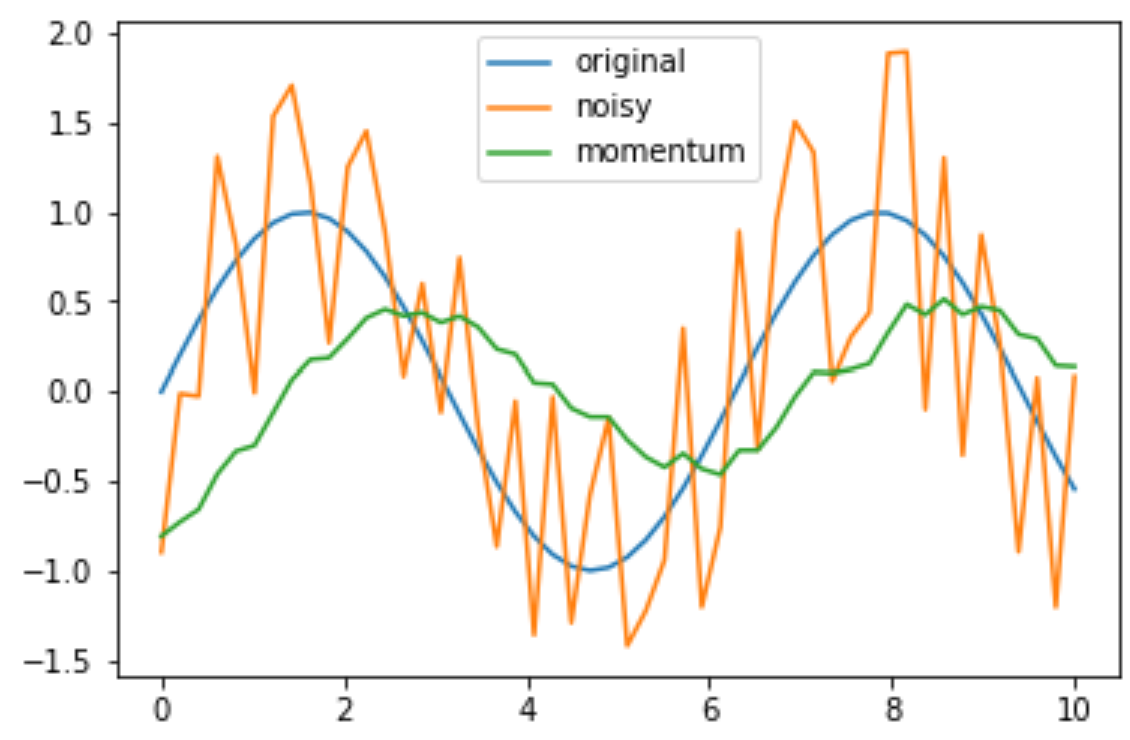
\includegraphics[width=\textwidth]{figs/momentum.png}
    \end{center}
    

\end{frame}

\begin{frame}
    \frametitle{Why is it called exponential moving average?}
\begin{align*}
    dw_t&=\beta dw_{t-1}+(1-\beta)\nabla_t\mathcal{L}\\
    &=\beta (\beta dw_{t-2}+(1-\beta)\nabla_{t-1}\mathcal{L})+(1-\beta)\nabla_t\mathcal{L}\\
    &=\beta^3dw_{t-3}+\beta^2(1-\beta)\nabla_{t-2}\mathcal{L}+\beta(1-\beta)\nabla_{t-1}\mathcal{L}+(1-\beta)\nabla_t\mathcal{L}\\
    &=\beta^{t-1}(1-\beta)\nabla_1\mathcal{L}+\beta^{t-2}(1-\beta)\nabla_2\mathcal{L}+\ldots+(1-\beta)\nabla_t\mathcal{L}
\end{align*}
    \begin{itemize}
        \item Usually $\beta<1$ so $a>b\Rightarrow \beta^a<\beta^b$
        \item Moreover, $n\rightarrow \infty\Rightarrow \beta^n\rightarrow 0$
        \item and $\beta=0\Rightarrow dw_t=\nabla_t\mathcal{L}$
    \end{itemize}

\end{frame}

\begin{frame}
    \frametitle{SGD with momentum}
    \begin{itemize}
        \item Validation accuracy vs epoch for ResNet18 with random initial weights
    \end{itemize}
    \begin{enumerate}
        \item SGD with momentum 0.9: pink
        \item Vanilla SGD: purple
    \end{enumerate}
\begin{center}
    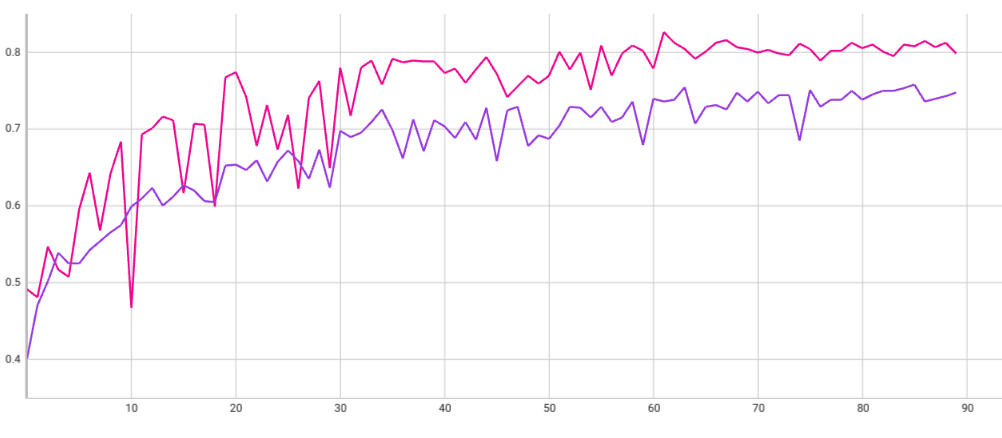
\includegraphics[width=\textwidth]{figs/with-without-momentum.png}
\end{center}
    

\end{frame}
\end{document}